%\documentclass[10pt, draft]{article}
\documentclass[10pt]{article}

\usepackage{fancyhdr}
\usepackage{multind}
\usepackage{pstricks}
\usepackage{graphicx}
\usepackage[yyyymmdd]{datetime}
\renewcommand{\dateseparator}{-}
\usepackage{geometry}
\geometry{letterpaper}
%
% Front Matter
%
\title{Arduino Sensor Network Documentation -- Hardware}
\author{Brent Seidel \\ Phoenix, AZ}
\date{ \today }
%========================================================
%%% BEGIN DOCUMENT
\begin{document}
\maketitle

\section{Synopsis}
This document contains descriptions of the hardware used in the Arduino Sensor Network.

\section{Network}
The network is based on the RS-485 standard.

\subsection{Topology}
The network uses a daisy-chained topology.  Each end of the chain should have a termination resistor of about 120$\Omega$.  One wire in the pair should have a pull up resistor to V$_{cc}$ and the other wire should have a pull down resistor to Gnd.  This is done at the controller node.

\subsection{Cabling}
The network cabling uses CAT-5 cables due to its easy availability.  It is not quite optimum for RS-485, but works for this application.  If your application pushes the limits more, you may need another solution.

\subsection{Connectors}
The cables are terminated with DE-9 connectors.  Pins 4 and 8 are used for the bus.  The other pins are avaialble.  Each node has 2 connectors so that the nodes can be daisy chained together.  The cables have male connectors and the nodes have female connectors.  Note that it might be simpler to use RJ45 connectors in your application.

\subsection{Interfacing}
The RS-485 drivers are p/n SN65HVD1781P from Texas Instruments.  Others will probably work, however it may simplify things if the same driver chip is used in all nodes.  It may also help you to get a quantity discount.  Since RS-485 is a differential bus, the drivers have two outputs called `A' and `B' or `+' and `-'.  One side goes high while the other side goes low.  Unfortunately, the labeling isn't completely consistent.  If you use the same driver throughout, you can just make sure that all the `A' sides are connected together and all the `B' sides are connected together.  If you mix drivers, you may need to do a little experimenting to make sure that the proper sides are connected.


\subsection{Baud Rate}
Since there is not a lot of data to transfer, a high baud rate is not necessary.  A higher data rate will put more of a processing load on the nodes and leave less time for them to process their data.  This is a bigger factor for the basic Arduinos.  My application uses 115.2kbps and it seems to work.  An oscilloscope shows that the waveform isn't too distorted.  It also don't put too heavy of a load on the nodes for this particular application.  If more processing is needed in the nodes, a lower baud rate may be needed.

\subsection{Backchannel}
It was decided that it would be useful to be able to send commands from the HTTP gateway (BeagleBone Black) to the controller.  To accomplish this, the TX side of the serial port on the BeagleBone Black and the RX side of one of the extra serial ports on the Arduino Mega 2560 were used.  Since the RS-485 drivers were purchased in bulk, there were some available.  Using these took care of the level shifting (3.3V to 5V) and any needed isolation between the two boards.

\section{Nodes}
There are three basic types of nodes in the network.

\subsection{Responder}
The responder nodes are either Arduino Unos or Boarduinos (an Arduino clone from Adafruit, p/n 72).  See Figure \ref{fig:basic} for an example basic connection of an Arduino Uno to the RS-485 bus and a sensor.  The responder nodes need at least a single serial port and should have an I2C port for interfacing with sensors.  Since the software is for Arduinos, it would need to be ported for any other platform.

\begin{figure}
  \centering
  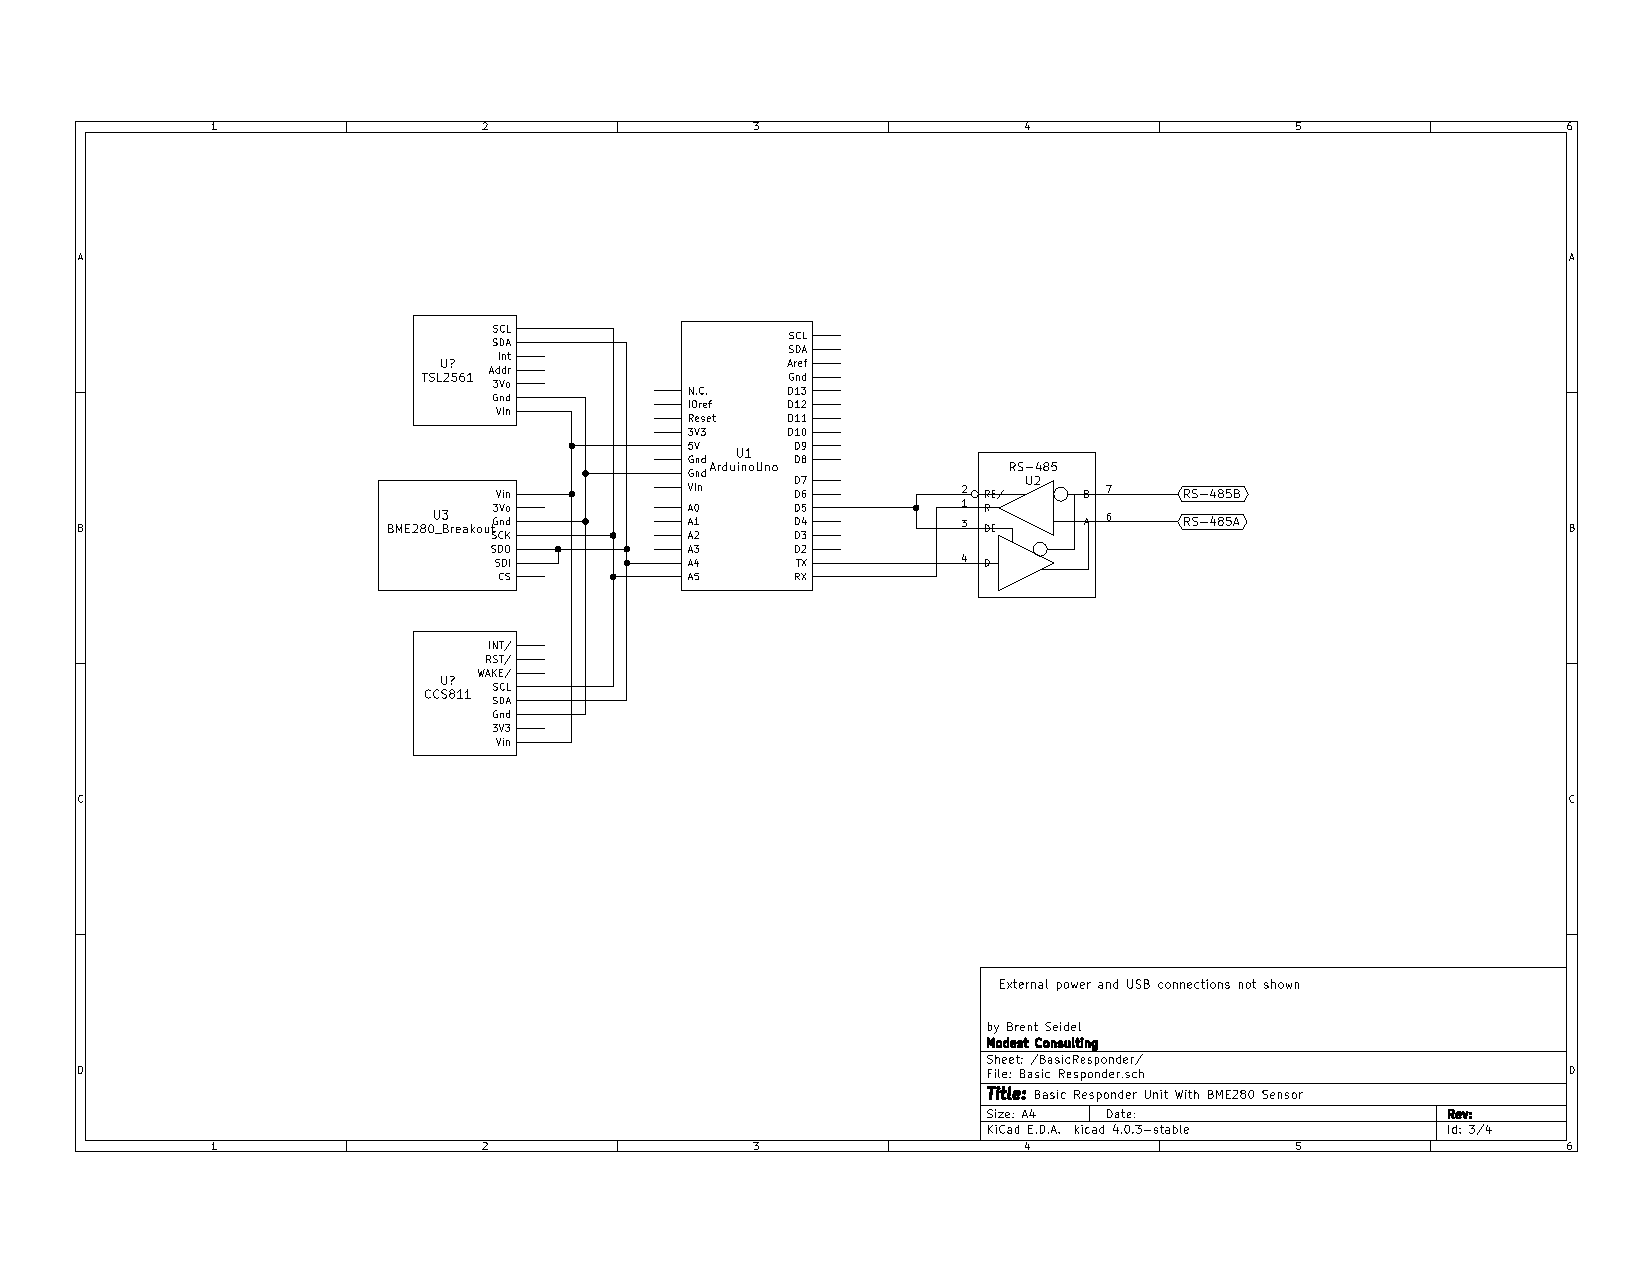
\includegraphics[width=\textwidth]{ResponderUnit.pdf}
  \caption{Basic Arduino Uno Responder Unit with BME280 Sensor}
  \label{fig:basic}
\end{figure}

\subsection{Controller}
The controller is an Arduino Mega 2560.  See Figure \ref{fig:controller} for an example controller node.  Note that the RS-485 interface on the controller contains the pull up and pull down resistors for the A and B wires.  The controller node needs at least two serial ports and possibly other interfaces if it is also to produce data.

\begin{figure}
  \centering
  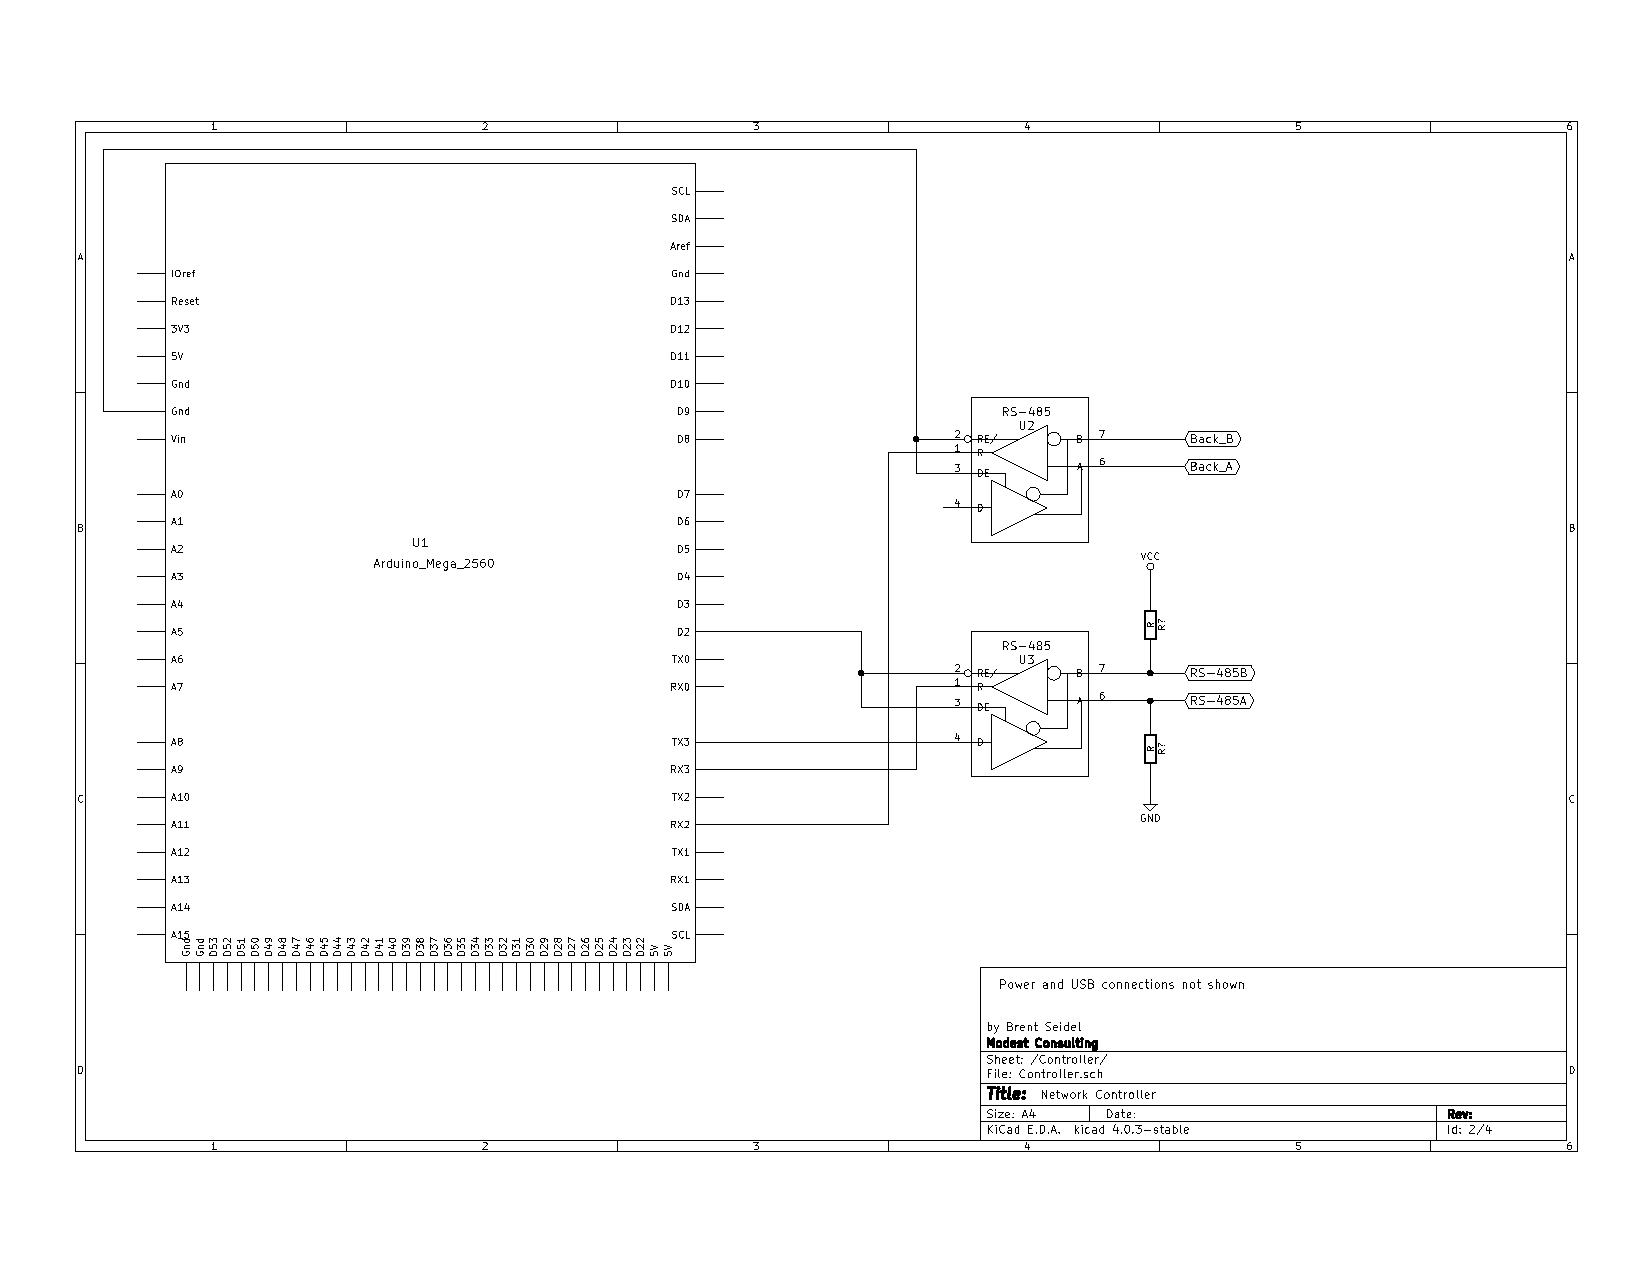
\includegraphics[width=\textwidth]{ControllerUnit.pdf}
  \caption{Controller Unit}
  \label{fig:controller}
\end{figure}

\subsection{Web Gateway}
The optional web gateway is a specialized form of listener.  It is based on the BeagleBone Black microcontroller.  See Figure \ref{fig:gateway} for an example web gateway node.  The HTTP gateway needs a serial port and an ethernet port.  The software is written in Ada 2012 and is based on Linux.  Any platform that supports this and has the required ports will probably work.

\begin{figure}
  \centering
  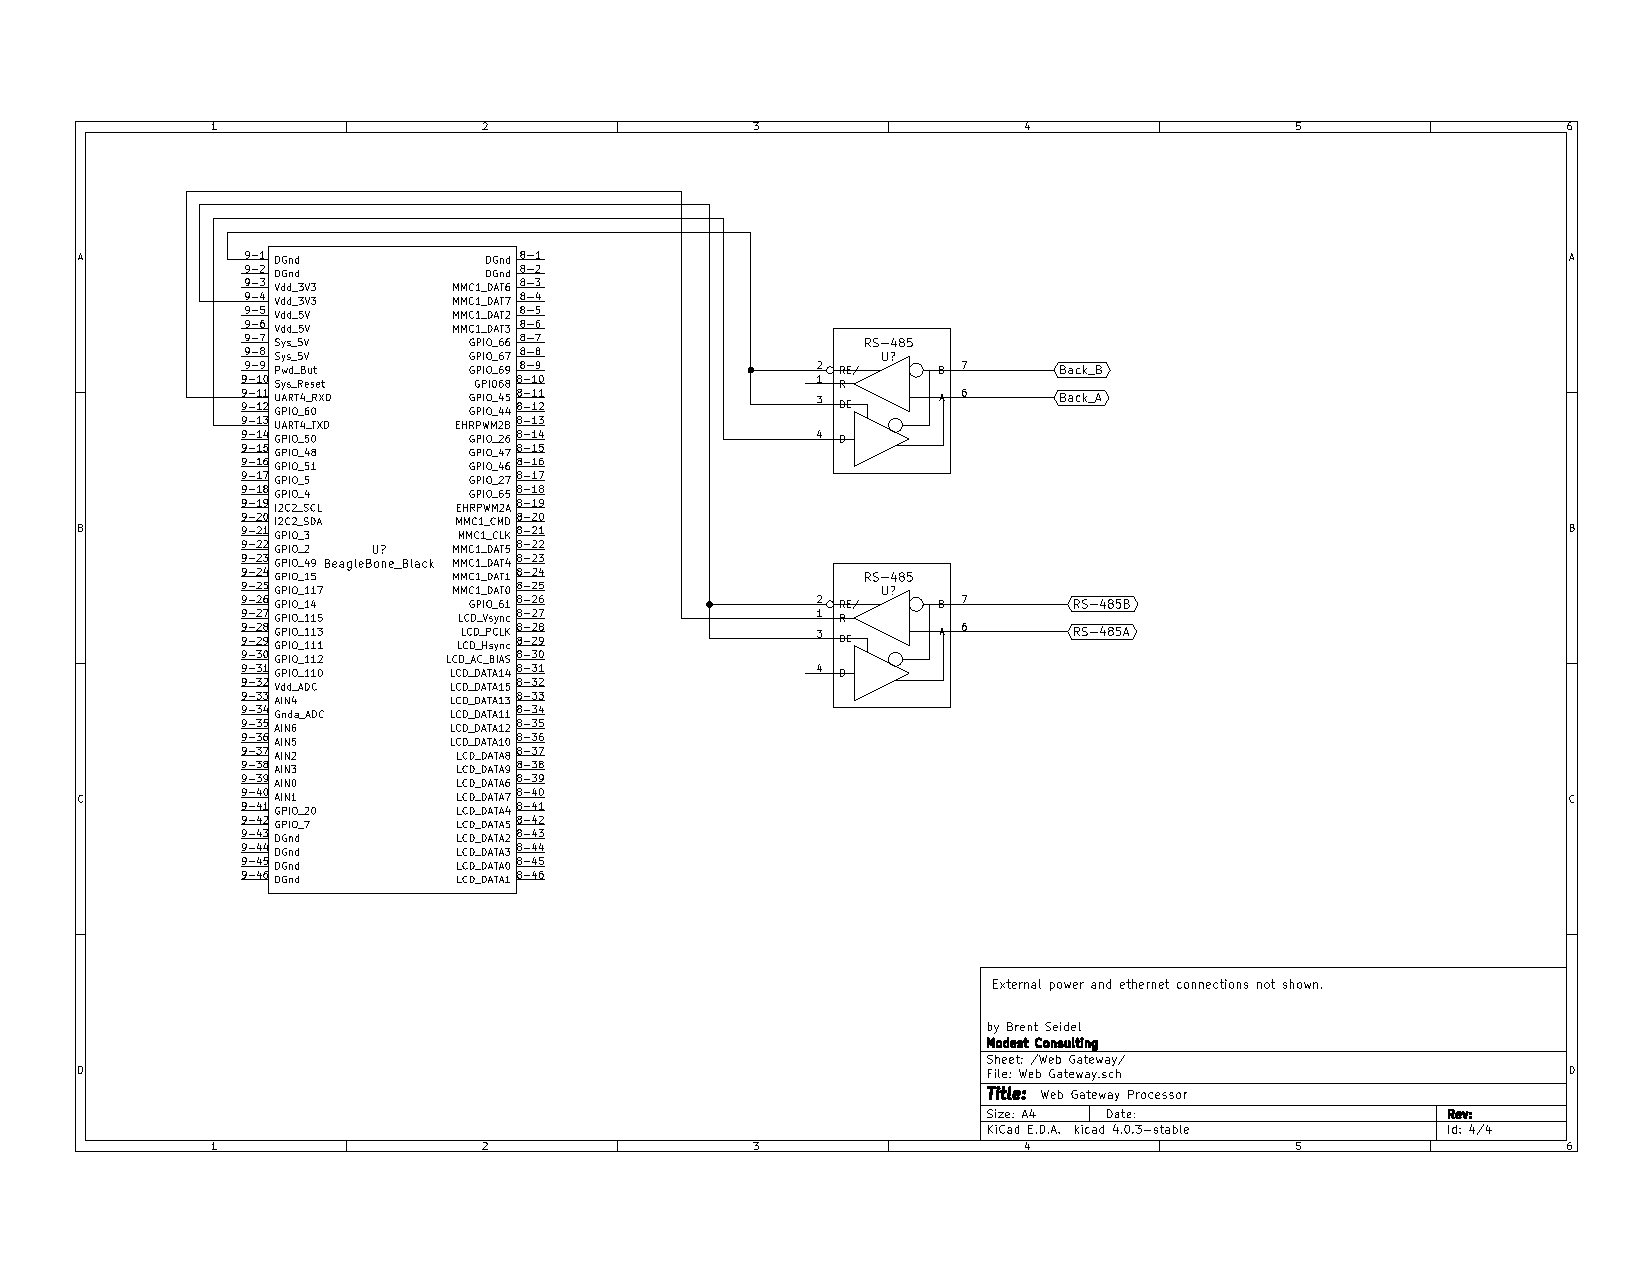
\includegraphics[width=\textwidth]{WebGateway.pdf}
  \caption{Web Gateway Unit}
  \label{fig:gateway}
\end{figure}



\section{Sensors}
The responder nodes can use the discrete I/O pins and the analog input pins.  Custom code is needed to produce the data on the bus.  Software is written for three different I2C based sensors:

\begin{itemize}
  \item BME280 (Adafruit p/n 2652) - This sensor provides calibrated temperature, barometric pressure, and humidity.
  \item TSL2651 (Adafruit p/n 439) - This is a digital light sensor that provides a reading of the light intensity.
  \item CCS811 (Adafruit p/n 3566) - This sensor provides uncalibrated CO$_2$ and Volatile Organic Compound readings.
\end{itemize}

\section{3D Printed Parts}
To be added once 3D models are added to repository.

\section{Miscellaneous}
In addition to the micro controllers, a few of other parts are needed.  The parts for the RS-485 network have already been mentioned.  The sensors needed depend on what you want to do.  Some other parts will be helpful.  A pack of 0.1'' female headers (Adafruit p/n 598) comes in handy when you want to be able to plug and unplug connections.  A set of ``perma-proto'' boads is handy for soldering up simple circuits.  These are also available from Adafruit in various sizes.  I mostly used 1/2 and 1/4 sizes.


\end{document}
